%%%%%%%%%%%%%%%%%% USAGE INSTRUCTIONS %%%%%%%%%%%%%%%%%%
% - Compile using LuaLaTeX and biber, unless there is a particular reason not to. Do not use the older LaTex/PDFLaTeX or BibTeX. (The fonts won't work correctly.)
% - Font and the report 'year' must be specified when all \documentclass or the template won't work correctly. (There's no error checking/default cases!)
% - For best performance save images/graphics as PDF files, not as png/jpg/eps. This makes no difference to how images are inserted using \includegraphics.
% - As many further packages as wanted can be loaded. Below are just an example set. Note that template itself loads a number of packages, including hyperref.
% - References are handed using biblatex.
% - Link to the presentation of theses policy: https://documents.manchester.ac.uk/DocuInfo.aspx?DocID=2863



%%%%%%%%%%%%%%%%%% META DATA SETUP %%%%%%%%%%%%%%%%%%
% This is where the document title and author are set. Other details for the title page are set later
\begin{filecontents*}{\jobname.xmpdata}
  \Title{Third Year Project Report - Blood Glucose Forecasting using Machine Learning} 
  \Author{10444901} % should be student number rather than name to help with annoymous marking
  \Language{en-GB}
  \Copyrighted{True}
  % More meta-data fielda can be added here if wanted, see https://ctan.org/pkg/pdfx?lang=en for fields
\end{filecontents*}


%%%%%%%%%%%%%%%%%% DOCUMENT SETUP %%%%%%%%%%%%%%%%%%
\documentclass[times,thesis]{uom_eee_dissertation_casson} 



%%%%%%%%%%%%%%%%%% PACKAGES AND COMMANDS %%%%%%%%%%%%%%%%%%

% Packages
\usepackage{graphicx,psfrag,color} % for postscript graphics files
  \graphicspath{ {./images/} }
\usepackage{amsmath}               % assumes amsmath package installed
  \allowdisplaybreaks[1]           % allow eqnarrays to break across pages
\usepackage{amssymb}               % assumes amsmath package installed 
\usepackage{url}                   % format hyperlinks correctly
\usepackage{rotating}              % allow portrait figures and tables
\usepackage{multirow}              % allows merging of rows in tables
\usepackage{lscape}                % allows pages to be typeset in landscape mode
\usepackage{tabularx}              % allows fixed width tables
\usepackage{verbatim}              % enhanced version of built-in verbatim environment
\usepackage{footnote}              % allows more control over footnote environments
\usepackage{float}                 % allows H option on floats to force here placement
\usepackage{booktabs}              % improve table line spacing
\usepackage{lipsum}                % for adding dummy text here
\usepackage{subcaption}            % for multiple sub-figures in a single float
% Add your packages here


% Optional: for adding alt-text to images:
%\usepackage{pdfcomment}            % for alt text for accessibility
% Then to add images use:
% \pdftooltip{\includegraphics[width=0.5\textwidth]{image.pdf}}{Alt-text here}
% This makes the text in the image non-select-able though (assuming it's a vector file)

% Custom commands
\newcommand{\degree}{\ensuremath{^\circ}}
\newcommand{\sus}[1]{$^{\mbox{\scriptsize #1}}$} % superscript in text (e.g. 1st)
\newcommand{\sub}[1]{$_{\mbox{\scriptsize #1}}$} % subscript in text
\newcommand{\sect}[1]{Section~\ref{#1}}
\newcommand{\fig}[1]{Fig.~\ref{#1}}
\newcommand{\tab}[1]{Table~\ref{#1}}
\newcommand{\equ}[1]{(\ref{#1})}
\newcommand{\appx}[1]{Appendix~\ref{#1}}



%%%%%%%%%%%%%%%%%% REFERENCES SETUP %%%%%%%%%%%%%%%%%%

% Setup your references here. Change the reference style here if wanted
\usepackage[style=ieee,backend=biber,backref=true,hyperref=auto]{biblatex}
% Note backref=true adds a page number (and hyperlink) to each reference so you can easily go back from the references to the main document. You may prefer backref=false if you need to stick strictly to a given reference style


% Fixes which can't be applied in the .cls file
\DefineBibliographyStrings{english}{backrefpage = {cited on p\adddot},  backrefpages = {cited on pp\adddot}}
  \renewcommand*{\bibfont}


% Add more .bib files here if wanted
\addbibresource{references.bib}





%%%%%%%%%%%%%%%%%% START DOCUMENT %%%%%%%%%%%%%%%%%%

% Don't edit these lines, title and author are automatically taken from the document meta-data defined above
\begin{document}
\makeatletter
\title{Third Year Project Report - Blood Glucose Forecasting using Machine Learning}
\studentid{10444901}
\makeatother

% Set the below yourself
\course{Computer Science}  % "Master of Science in" is added automatically
                                                   
\submitdate{2023}                                  % regulations ask only for the year, not month
\wordcount{10000}                          % use \wordcount{} to set the count, \thewordcount to print in the text
\maketitle


%%%%%%%%%%%%%%%%%% LISTS OF CONTENT %%%%%%%%%%%%%%%%%%
\uomtoc% other lists are not required, but can include \uomlof and \uomlot if really want to


%%%%%%%%%%%%%%%%%% ABSTRACT %%%%%%%%%%%%%%%%%%
\begin{abstract} % put abstract here. Limit is 1 page.
  This is abstract text. 
  
\end{abstract}%
\clearpage

%%%%%%%%%%%%%%%%%% SECTION 1 %%%%%%%%%%%%%%%%%%
\section{Introduction}

  \subsection{Background and motivation}
    Talk about diabetes generally, can take from introduction of lit review

    Type 1 Diabetes Mellitus (T1DM) is a life-long autoimmune disease that typically manifests itself in children between 10 and 14 years of age. That is not to say, however, that a diagnosis of T1DM is restricted to those individuals within this age range, and whilst it is rare for diagnosis to be made in individuals over 40, it is possible for a diagnosis of T1DM to occur at any age. T1DM is characterised by the destruction of the beta-cells within the pancreas which are responsible for producing insulin \cite{t1d}, a hormone used  by the body to help blood glucose to be absorbed by cells to be used for energy \cite{insulin}, and to store blood glucose for later use. This loss of insulin producing beta cells means that there is an inability for T1DM patients to regulate their own blood glucose levels, which if left untreated can lead to hyperglycemia (blood glucose levels being too high). As such, T1DM patients are reliant on the subcutaneous injection of synthetic insulin to control the glycemic levels in their body and to maintain a healthy blood glucose level. Diagnosis of the condition is based on hyperglycemia, with a fasting blood glucose concentration above 7.0 mmol/L being characterised as enough to diagnose. Other symptoms commonly seen before diagnosis are going to the toilet a lot, constantly being thirsty, and weight loss \cite{t1dcauses}.

    In order to calculate how much external insulin to inject, and thus avoid hyperglycemia and hypoglycemia (blood glucose levels being too low), T1DM patients must keep track of how much glucose they ingest and dose themselves with a corresponding volume of insulin. This counting and dosing process is not an exact science, and being inaccurate can lead to potentially life-threatening situations for patients. As such, technology has been introduced to make the process easier. Continuous Glucose Monitoring (CGM) devices \cite{pumpcgm} provide real-time information on someone's current Blood Glucose (BG) levels, whilst insulin pumps exist that are capable of slowly providing insulin over a long period of time, rather than having a single large dose given by injection pen. This new technology has greatly improved the lives of many patients, and there is hope that new technology can continue to do the same. One of the main issues with current technology is that whilst it is able to immediately detect issues with current BG levels, there is still a response time between corrective actions being taken and their impacts on BG levels. This response time has lead to much research being done into predictive algorithms that could inform a patient ahead of time of any issues that may occur, allowing them to react with ample time and avoid any high/low blood glucose levels before they even manifest. One such branch of these predictive algorithms is machine learning algorithms and an exploration of this topic will form the basis of this project report.
  
  \subsection{Aims and objectives}
    This project aims to investigate and implement machine learning methods to perform blood glucose prediction, then compare and contrast the performance of these different methods.

    To guide the development of the project, the following objectives have been identified: 
    \begin{itemize}
        \item Obtain, understand and configure a suitable Continuous Glucose Monitoring (CGM) dataset.
        \item Perform a literature review on existing approaches taken to perform blood glucose prediction.
        \item Implement a selection of the researched approaches.
        \item Experiment with hyperparameters on different approaches to try and achieve optimal accuracy for the approach as stated by scientific metrics.
        \item Experiment with the different approaches over varying prediction horizons.
        \item Produce visualisations to view the performance of the different prediction techniques over differing time horizons.
        \item Analyse and compare the effectiveness of the different approaches blood glucose prediction.
        \item Discuss the work that would need to be done to make such prediction technologies available and useful to real patients.
    \end{itemize}
    
  \subsection{Report structure}
    In this report, there is first a short literature review to gain insight into existing machine learning techniques for BG prediction as well as their respective performances. A few approaches are then selected from those researched, and the development and optimisation process of the different models is discussed and documented. Once finished, the models are experimented with and the data produced is visualised in the report. Finally, conclusions and insights into future work are drawn from the visualisations presented.
    
%%%%%%%%%%%%%%%%%% SECTION 2 %%%%%%%%%%%%%%%%%%
\section{Literature review} % edit section heading as appropriate
    \subsection{Introduction}

    It is important to note that when measuring BG levels, there are two prevalent units - mmol/L which is used in the UK, and mg/dL which is used outside of the UK. The conversion ratio between the two is 18mg/dL : 1mmol/L. According to the World Health Organisation (WHO), blood glucose levels should be between 3.9 mmol/L and 5.6mmol/L \cite{WHOBGL} for ordinary people and between 5 mmol/L and 9 mmol/L for diabetic patients.   As a result of this, there is a constant need for diabetics to manage their blood glucose levels, with the aim of spending as much time within this range as possible and avoiding hyperglycemia and hypoglycemia. Both hyperglycemia and hypoglycemia are serious conditions that can lead to life threatening situations for patients; making precision when managing blood glucose levels a matter of life and death. Patients who spend extended periods of time in a hyperglycemic state can suffer from kidney damage, nerve damage (neuropathy), damage to the blood vessels of the retina leading to blindness, and complications with bones and joints. In extreme cases of hyperglycemia, diabetic ketoacidosis (DKA) can occur, which, if left untreated, can lead to a life-threatening diabetic coma \cite{mayohyper} Meanwhile, hypoglycemia affords a range of different issues, ranging from slurred speech and numbness to seizures, coma and death in extreme cases if left untreated\cite{adahypo}. 
    \newline
    With an estimated 422 million people worldwide suffering from diabetes \cite{world_2019}, making it the 3rd most common chronic illness in the world, it is clear that there is a need, and a great benefit to be gained, from using technology to help patients more accurately manage their blood glucose levels. Unfortunately, regulating blood glucose levels is not an exact science, and there are a myriad of different factors that can impact a patient's blood glucose levels \cite{bglfactors}. The predominant factor is carbohydrates ingested by the patient. Carbohydrates are broken down by the amylase enzyme into glucose which is transferred into the blood stream to be absorbed by cells; clearly having a direct impact on the levels of glucose in the blood. Other major factors include any physical activity done by the patient, and any external insulin taken by the patient. Whilst these factors are more easily measurable for patients, and thus can be adapted to and controlled, other factors such as stress, illness and injury, and hormonal changes can also have a substantial impact on regulating blood glucose levels, whilst being much more difficult to manage. This makes the task of predicting how blood glucose levels will change and respond accordingly difficult for T1DM patients and machines alike - one small change can lead to large variations in behaviour.  

    The end vision of diabetes related technology is known as the Artificial Pancreas (AP) and consists of a fully closed-loop system where a T1DM patient would have to do no management of their blood glucose level at all; the AP would handle everything. Some AP systems currently exist, both as home-brew systems and regulated healthcare systems \cite{apsystems} but these systems operate in a hybrid manner, and still require some level of input from the user. Unfortunately, due to the problems in variation and some other issues we will cover below, the creation of a completely hands-free AP system still seems to be far in the future. However, that is not to say that technology has had no impact on the lives of T1DM patients, as there have been many advances which have made noticeable impacts on improving the quality of life of patients. Introduced in 1985 \cite{diatech}, insulin pens are devices that allow patients to inject insulin directly into their body. Coupled together with small, easy to use glucometers which were introduced in the 1980s, patients were able to frequently monitor their blood glucose levels, and respond accordingly by either using their insulin pens, or ingesting more glucose, to control their blood glucose levels. \begin{figure}[H]
        \centering
        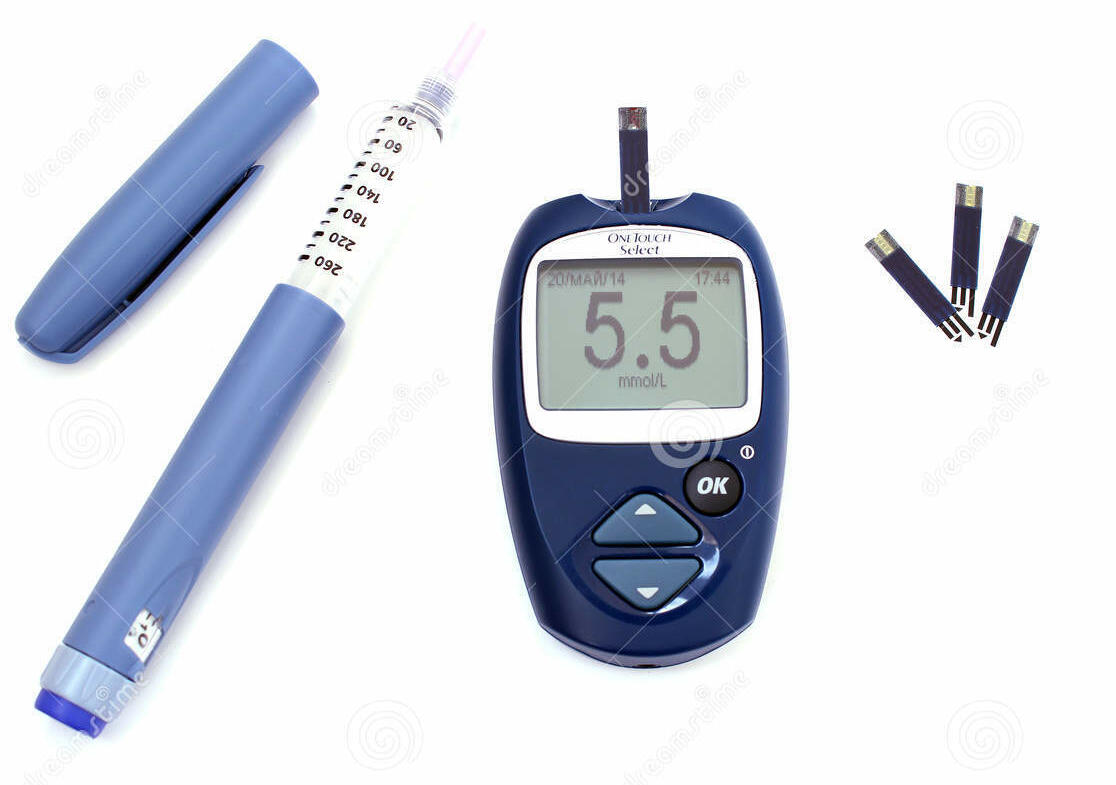
\includegraphics[width=0.5\textwidth]{images/glucometer.jpg}
        \caption{
         An image showing a modern insulin pen and glucometer \cite{penandglucometer}
        }
    \end{figure}
    This method of self-monitoring of blood glucose (SMBG) has significant drawbacks as blood is sampled intermittently, providing only short insights of glucose concentrations, whilst ignoring ongoing glucose fluctuations. With the idea of being able to monitor blood glucose at all times, Continuous Glucose Monitoring (CGM) devices were introduced that measure glucose concentrations at intervals (usually between 1-5 min), and then transmits/stores those values. Alongside the invention of the insulin pump, a device that allows programmable infusions of insulin over long, or short, periods of time, diabetic patients were given a much more reliable way of constantly monitoring and regulating their blood glucose levels.
    \begin{figure}[H]
      \centering
      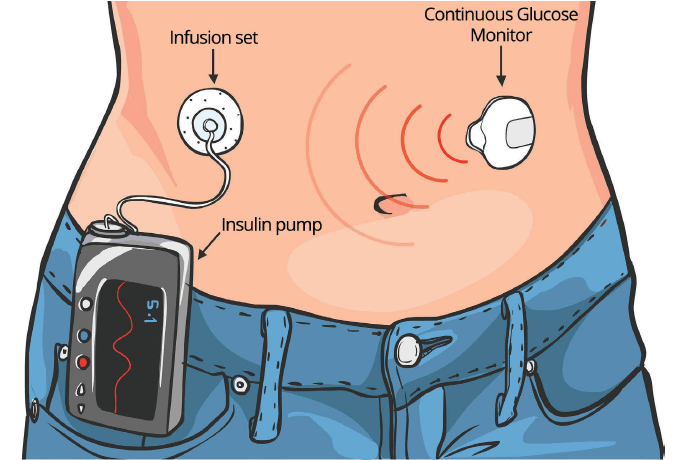
\includegraphics[width=0.5\textwidth]{images/CGMPump.png}
      \caption{
       A diagram showing the interaction between a CGM and insulin pump\cite{pumpandmonitor}
      }
    \end{figure}
    
    The creation of CGM devices also lead to a new capability - the ability to create blood glucose datasets by accessing the data stored in the CGM; datasets which are needed to train accurate Machine Learning (ML) models. It is clear that the capability to accurately predict when one might suffer a hyperglycemic, or hypoglycemic, episode would be invaluable to a T1DM patient, as it would allow them to behave proactively to prevent the episode from ever occurring, rather than the current reactionary method, which requires a hypo/hyperglycemic episode to be taking place before we can detect its presence. We name the amount of time into the future which we forecast the Prediction Horizon (PH). Current prediction horizons available to T1DM patients are very short, and thus don't give ample time for patients to react to predicted issues. Current CGM devices are capable of crude alarm systems that can inform patients if their BG levels are steeply dropping or rising, but once again this is just a reactionary measure. As such, much work has been done in applying ML techniques to improve the length of the PH to a length of hours instead of minutes, but as of yet no concrete solution to the problem has been found. This is due to a variety of reasons, such as the variability of a patient's BG level, due to day-to-day uncontrollable factors as mentioned earlier, as well as some other issues that will be discussed later when different approaches that have been experimented with to solve this very problem are explored.

	\subsection{Detail}
    \subsection{Machine Learning}
      Add section about papers / machine learning in general. Will consider whether to put ML here or later on.

      Machine learning is a field of Artificial Intelligence that focuses on learning through observing patterns in large quantities of past data, and iteratively improving accuracy at a given task \cite{whatisml}. In the context of T1DM, the large quantities of past data refer to the patient's blood glucose levels over a period of months (as well as other points of interest such as exercise undertaken / carbohydrate intake / insulin intake), whilst the task to improve at is predicting the BG levels of the patient for a specified PH. There is interest in the use of Artificial Neural Networks (ANN), a kind of Machine learning model that is able to learn very complex relationships between data \cite{whatisnn}. ANNs are based off of the functioning of the human brain, and are capable of modifying their structure to suit the task at hand. They consist of a number of nodes and a corresponding number of connections which link one node to another, where each connection has a weight which signals how strong the connection between the two nodes is. An ANN can consist of many layers with the first and last layers being known as the input and output layers respectively. Any layers inbetweeen the two are called hidden layers. Each node has an input into it, and in the final layer of the network, an output is given. At each node, every input is multiplied to its corresponding weight, and an activation function is applied to sum of these values to generate the output value to be passed to the next layer of the network. An activation function is a function that transforms the output in some way - for example the binary step activation function checks if the value is above a given threshold. If so, the node outputs 1, otherwise 0.
      \begin{figure}[H]
        \centering
        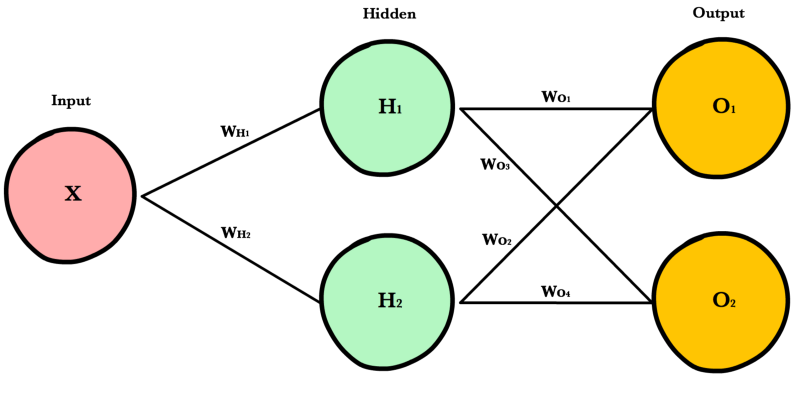
\includegraphics[width=0.5\textwidth]{images/basicNN.png}
        \caption{
         A diagram showing the nodes, connections and weights of a simple ANN \cite{whatisnnimage}
        }
      \end{figure}
      In order for the NN to learn the task at hand, we define an error function between the actual output of a given input and the output generated by our network. This error function can be specified to suit the model as needed and it is common, in the case of blood glucose forecasting, to see an error function comparing the absolute difference between predicted blood glucose levels, and real recorded blood glucose levels. Through an iterative algorithm such as gradient descent \cite{whatisgd}, whereby we calculate the derivative of the error function and attempt to iteratively adjust the network weights to reach the minimum value of this function, the ANN can learn very complex relationships between the data input into it and the expected outputs. 
      \begin{figure}[H]
        \centering
        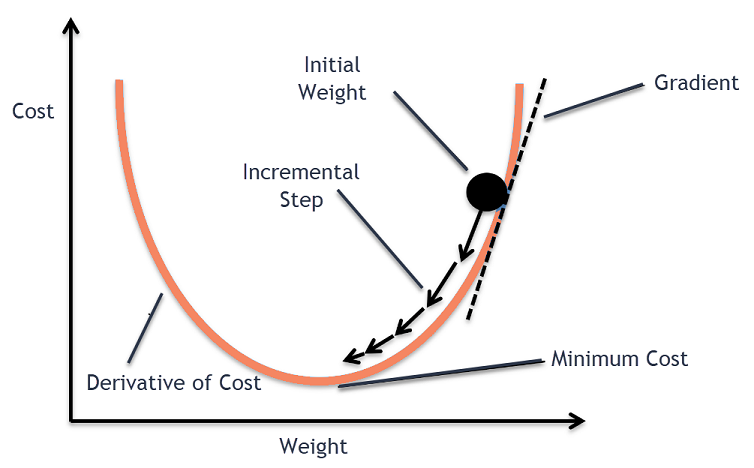
\includegraphics[width=0.5\textwidth]{images/gradientdescent.png}
        \caption{
         A visualisation of the gradient descent process\cite{whatisgdimage}
        }
      \end{figure}
      Much work has been done researching the applications of different kinds of ANN to blood glucose forecasting, as it was believed that not only would ANNs be able to provide very accurate predictions on future BG levels, but also would be able to solve the problem of inter-subject variability - by training a new network on each individual patient's BG data. 

      As will be seen below, when training neural networks, there is much debate amongst researchers about what to include and what not to include within the input parameters to the network. Some believe that just the CGM data is sufficient, claiming that the inclusion of other measures, such as carbohydrate intake, would simply increase variance and decrease model performance. This is sharply contrasted by researchers who have experimented with both complex and simple physiological models to try and model the effect that factors such as exercise and insulin intake will have on future glucose levels. There is much debate about the correlation between past glucose levels and future levels, with some using only the current blood glucose levels as an input to the model, and others using many past readings to inform future predictions. Whilst there is much diversity amongst the methods employed, unfortunately, the overarching theme from most ANN approaches is that they can be very accurate at shorter PH (~30 minutes), but that accuracy quickly drops off at larger PH (~6 hours). Moreover, the vast majority of work done has been in silico, and such prediction methods are yet to be rigorously tested on patients in their day-to-day lives.

      \subsection{Simple ANN Approaches}

      One such example of the application of NNs to the task of blood glucose prediction was by Pérez-Gandía et al.\cite{paper3}, who attempted to use a NN trained using only CGM data. The model considered the preceding 20 minutes of CGM data and attempted to predict BG levels at 3 different PHs of 15, 30 and 45 minutes. The accuracy of the model was measured using a number of different metrics. One such metric is the Root Mean Squared Error (RMSE) - a widely used metric for BG prediction models that takes the square root of the sum of the squares of all prediction errors.
      \[RMSE = \sqrt{\frac{\Sigma_{i=1}^{N}{\Big(Predicted_i - Actual_i\Big)^2}}{N}}\]
      Another metric used was the Prediction Delay (PD) - a metric that takes into account the delay between when certain features of the CGM data were seen in the original data and the predicted data (for instance the time gap between a peak appearing in the original and predicted data). When making a prediction, two different approaches were compared - a standard ANN model that would make one prediction across the PH, and an AutoRegressive Model (ARM). In an ARM, the model makes the prediction one step at a time and uses a recursive algorithm to allow each prediction to inform subsequent predictions, trying to capture the relationships between previous and future BG levels more accurately. It was found that across the 15, 30 and 45 minute PHs their ANN model achieved a RMSE of ~10, 18, 27, mg/dL respectively. To analyse these results, we introduce the notion of an 'accurate prediction' which, by using the accuracy of glucose sensors \cite{CGMacc}, we define to be a prediction within 15 mg/dL (0.85 mmol/L) of the actual value.  For the short PH of 15 min, these results are quite promising and accurate, but this accuracy very quickly falls off. For upward trends (when the patient enters hyperglycemia rapidly) in the data, there was a PD of 4, 9 and 14 minutes respectively, and for downward trends (when the patient enters hypoglycemia rapidly), a PD of 5, 15 and 26 minutes was seen. Whislt the PD is worse when detecting downward trends, these results are still promising as at the 45 min PH, a patient would still have a 31 min period to react to an upward trend, which would give them ample time to make corrective action.

      This use of a basic NN highlights some of the main problems with this approach when applied to blood glucose prediction. First, the accuracy falls of very quickly, with 2.7 times worse performance over a short difference in time of 30 minutes, and second is that the model is much quicker at recognising upward than downward trends. This is a major issue, as downward trends lead to hypoglycemic episodes, which can be far more dangerous in the short term than hyperglycemic episodes. In the case of this model, the 26 min PD at a 45 min PH would give some warning, but still wouldn't give a patient ample time to take corrective action. To try and combat the first of these problems, Alfian et al. \cite{paper5} included time-domain attributes along with their model. Time-domain features of the past CGM data such as minimum, maximum, mean, standard deviation etc. are passed as inputs to the model along with the data, in the hopes of improving accuracy. The approach was tested with the data of 12 different patients, across different PHs of 15, 30, 45 and 60 minutes. The accuracy found varied from patient to patient, with the best patient having RMSE values of 1.42, 3.61, 6.22 and 8.03 mg/dL respectively across the PHs and the worst obtaining values of 4.72, 11.32, 16.88 and 26.65 mg/dL respectively. The accuracy on the best patient is incredibly promising. A clinically acceptable BG prediction is stated to be one within 20\% of the reference value \cite{CEGA}, which would mean that with a RMSE of 8.03 mg/dL at 60 min PH, and with typical BG levels being between 120 mg/dL and 162 mg/dL \cite{WHOBGL} this model is providing clinically acceptable and accurate predictions 1 hour into the future. With this in mind, we denote the term of a clinically acceptable prediction error to be one that is within a 20\% range of 120, or one that is below 24 mg/dL (1.5 mmol/L). Whilst this model is a great improvement on the basic use of a NN, the difference in accuracy between the best and worst patients highlights the large performance variability - a variability that could result in medical emergencies if used currently without proper in vitro testing.

      \subsection{RNN Approaches}
      \subsubsection{RNNs}
      Another method to try and better capture the relationship between previous CGM readings and future expected readings is a specific type of NN called a Recurrent Neural Network (RNN) \cite{whatisrnn}. An RNN differs from an ordinary 'feedforward' ANN in the sense that in an ANN, all inputs are passed from the input layer 'forwards' through each layer until they reach the output layer. By contrast, an RNN implements a 'loop-like' structure. The inputs are recursively passed into the network such that the value at a node in the network depends on both the current input and a hidden representation, which is calculated by all the previous inputs to the model. In this way, RNNs offer a way to calculate compound representations that depend on all the previous inputs to the network, rather than just passing in and handling the previous CGM data as separate datapoints. 
      \begin{figure}[H]
        \centering
        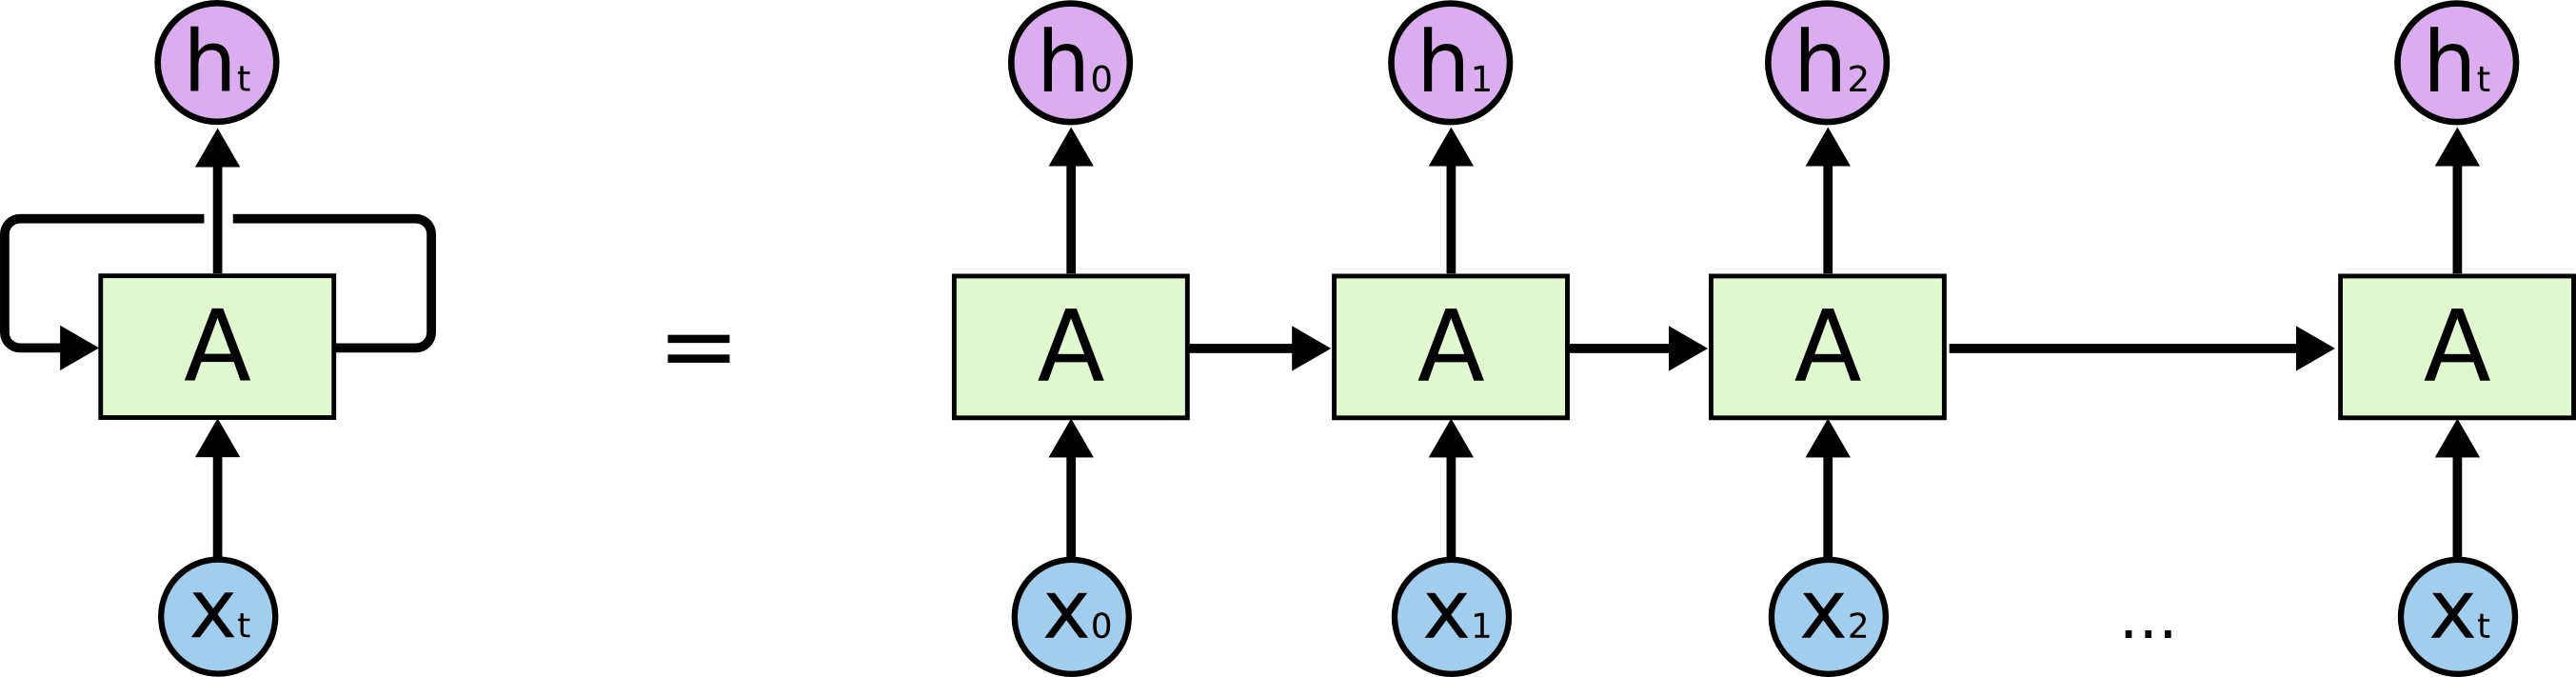
\includegraphics[width=0.5\textwidth]{images/basicRNN.png}
        \caption{
         A diagram showing the 'looped' structure of an RNN \cite{whatisrnnimage}
        }
      \end{figure}
      The most often seen implementation of RNNs is the Long Short Term Memory (LSTM) RNN, which, at each node in the network, implements an input, output and forget gate to control the value of the recursive hidden representation \cite{lstminfo}. The forget gate controls what information from the previous hidden representation we keep, the input gate controls which information from the current input we add, and the output gate controls what information we pass to the next loop of the and would definitely provide some benefit to T1DM patients network as the next hidden representation. The values of these gates are iteratively updated during the training process to obtain the best accuracy. 
      \begin{figure}[H]
        \centering
        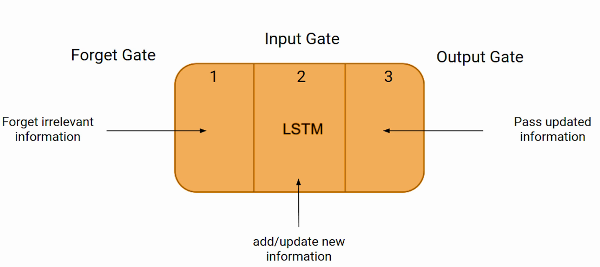
\includegraphics[width=0.5\textwidth]{images/basicLSTM.png}
        \caption{
         A diagram showing the functions of the different LSTM gates \cite{lstminfo}
        }
      \end{figure}
      These gates control the value of the hidden representation in such a way that it avoids the problems of exploding/vanishing gradient; a major issue with traditional RNN networks, where exceptionally large/small values of gradients when updating weights in the network. This leads to issues when training where either the updates to weights become far too large or far too small to result in any real performance improvement for the network.

      \subsubsection{RNNs for Blood Glucose Prediction}
      Robertson et al. \cite{paper1} used RNNs to perform BG prediction on data generated from the Artificial Intelligence Diabetes Assistant (AIDA) diabetes simulator \cite{AIDA}. AIDA is a freeware diabetes simulator that models steady-state glucose-insulin interactions by describing the physiology of a person with T1DM. This model considers carbohydrate intake, insulin, kidney function and insulin sensitivity. Predictions were made on the data for both short (15-60 minutes) and long term (8-10 hours) PHs. Some points of note viewed from their experiment were that in short term prediction, there were errors between the predicted and actual Blood Glucose Levels (BGL) of over 1 mmol/L - an amount that is not only inaccurate by our measure of accuracy, but also very unsafe in practice. It was also noted that predictions directly after input events (e.g. meal eaten, insulin taken) were much less accurate; showing that the model wasn't able to correctly handle these events as it should. The model was also seen to be far more accurate at night, most likely due to the lack of events such as eating meals, which would lead to a dramatic change in BGL that the model cannot accurately predict. Overall, in the short term a RMSE of $0.15 \pm 0.04$ SD mmol/L was viewed and in the long term a RMSE of $0.14 \pm 0.16$ SD mmol/L was seen - again we note the trends that the model is far more unpredictable at longer term PH. Whilst these results are very promising, and accurate predictions are generated even at a longer term PH, it is also important to consider that the data was obtained in silico from a mathematical model, and so is not hugely indicative of performance on real life data. The mathematical model only handles a few variables to enact changes on its output BGLs, whereas in free-living conditions there are many more factors, such as stress levels and illness, whose fluctuations can impact BGLs in real-life patients.
      
      The model developed by Robertson et al., was limited, performing poorly when significant events are taking place, such as the ingestion of carbs and/or insulin being delivered, which can result in rapid changes in BGL. This is a common issue in the research of BGL prediction and whilst some believe that by studying just trends in the CGM data of a patient to implicitly identify when events like this take place, and change our predictions accordingly, there is a separate approach of using Compartmental Models (CMs) \cite{CMS} to directly input the data of these events (to include carbohydrate and insulin data) into the network. CMs are mathematical functions that try and describe the processes that occur in the inaccessible parts of the human body. For instance, you would have one model describing how the carbohydrate intake at a given time would impact blood glucose levels over a given period of time afterwards. These CMs can range from simple bell curves to much more complex models such as Hovorka's model \cite{hovorka}, and there has been research done into the benefits and drawbacks of using simple or more complex CMs. 

      Mougiakakou et al. \cite{paper4} proposed a solution for Blood Glucose Forecasting involving the combination of CMs and RNNs. The input data is passed to three separate CMs, which estimate 1) the effect of short acting insulin intake, 2) the effect of fast acting insulin intake, and 3) the effect of carbohydrate intake on blood glucose levels. The outputs of these three CMs are then passed to the RNN along with past CGM data in order to predict subsequent blood glucose levels. Another point of note in this approach is that the RNN is trained with a Real-Time Recurrent Learning (RTRL) algorithm. Ordinarily, when training a network, you optimise the weights with a learning algorithm on a set of training data, then use those pre-determined optimised weights whenever making a prediction. Conversely, with Real Time Learning (RTL), the weights of the network continue to be improved during use, and each pair of predicted and real BGL values is used to iteratively update the network in real-time. This is thought be very applicable to BGL prediction, as you would be able to initially train a model on a batch of patient data, then continually improve the model as it was being used by the patient; permitting the model to become as personalised and accurate as possible for the user. The data for this model consisted of only 4 or 5 glucose measurements per day, over a period of ~70 days, making the data far sparser than that which has been seen in previous approaches. Overall, the approach obtained a RMSE of 41 mg/dL for predictions for each measurement; an impressively accurate result given the sparsity of the data, but a result that is neither particularly accurate nor clinically acceptable for use in vitro. Mougiakakou et al. \cite{paper4} concluded that including other information in the model such as sex, age, and number of years a patient has had the condition could improve the performance of the model. Of specific interest was the potential inclusion of more CMs to capture patient physical activity.

      The approach seen by Mougiakakou et al. \cite{paper4} used relatively complex, pre-defined mathematical models to describe the effects of the attributes that the CMs used were modelling. Munoz-Organero et al. \cite{paper6} attempted a different, more complex approach to the formation of their CMs, by training Deep Neural Networks to predict the impacts of Fast Insulin, Slow Insulin and Carbohydrate Intake on blood glucose levels. The output of these three models would be concatenated and fed as an input along with CGM data to give an overall prediction on the BG variation over the next time step. The deep physiological models were trained using 9 hour windows of data, and attempted to learn the BG variations over the time period, based on the three separate factors highlighted. It was noted that one of the key detriments to this kind of approach is the inconsistency of CGM datasets - some will note down every time a patient has a meal or takes insulin, whereas others will miss datapoints, which can lead to inaccuracies in the model. The models were trained and tested using data from both the AIDA diabetes simulator and the open source D1NAMO dataset \cite{dinamo} (an open-source dataset collected from nine real life T1DM patients). Across a 30 minute PH, the model on the D1NAMO dataset achieved a RMSE of 6.42 mg/dL and with the simulated AIDA data, a RMSE of 3.45 mg/dL. These results show that the model was incredibly accurate over the data, with the AIDA data being the more accurate - as expected due to the added variability of real patient data. However, this accuracy is on data generated by healthy patients, and the dynamics of insulin/carbohydrate absorption would change massively due to factors such as stress and illness. This means that, in practice, such complex deep physiological models could become very inaccurate during these times of imperfect health, and thus still are unproven and unsafe for use by real T1DM patients. It would require more real-life testing to verify whether this approach could feasibly work. Unfortunately, in practice, it is very hard to perform real life testing due to a number of factors such as obtaining ethical approval, finding a volunteer pool large enough to give accurate results and making sure that those volunteers adhere to the rules of the study correctly.

      Whilst directly modelling the impacts of other factors such as carbohydrate intake with CMs is possible, there is another train of thought that we should be able to intrinsically detect these events and their impacts by looking at different signals in the CGM data. One example of this approach was taken by Wang et al. \cite{paper8} who combined Variational Mode Decomposition (VMD) with an LSTM RNN optimised by Improved particle Swarm Optimisation (IPSO) to perform BG prediction. Imagine, for example, that a given T1DM patient eats lunch between 12-2 pm every day - we would expect to see a spike in their BG levels around this time of day every day. Through signal decomposition techniques such as VMD, we can extract the separate signals that combine to make the overall BG graph - in this case, one such signal would be a signal with a period of 1 day and a spike around the lunch time of the patient. Through this decomposition, it is thought to be possible to reduce the non-stationarity of the CGM data, and make it possible for the RNN to make more accurate predictions. To ensure the LSTM has optimal hyper parameters, Wang et al. \cite{paper8} employed an Improved Particle Swarm Optimisation algorithm - an algorithm that uses many 'particles' initialised at random points in the parameter space, then iteratively converges to the optimal solution by tracking the best particles in the current space, and initialising the next round of particles to be closer to these best ones.

      To measure the success of their approach, Wang et al. \cite{paper8} used both the RMSE between predicted and actual BG levels, as well as the Clarke Error Grid (CEG) \cite{CEGA}. The CEG is a tool for checking the accuracy of blood glucose monitors. It splits predictions into 5 separate zones: A, B, C, D and E. Zone A is defined as clinically accurate; Zone B indicates an incorrect, but benign, and therefore clinically acceptable prediction. Zone C represents values leading to inappropriate treatment, but without dangerous consequences for the patient. Zone D represents values leading to potentially dangerous failure to detect hypo or hyper-glycemic events and Zone E represents values leading to treat hypoglycemia instead of hyperglycemia and vice-versa. For a model to be clinically accurate, predictions should occur within zones A and B. Across a 30, 45 and 60 minute PH the model achieved an RMSE of 3.031, 5.432 and 5.716 mg/dL respectively. At the 60 minute PH, the model had 95.4\% of predictions in Zone A, 3.8\% in Zone B and 0.8\% in Zone D of the CEG. These results at are very promising, but the model is so far untested at the more important very long term PHs that are currently struggling to be accurately predicted over.

      \begin{figure}[H]
        \centering
        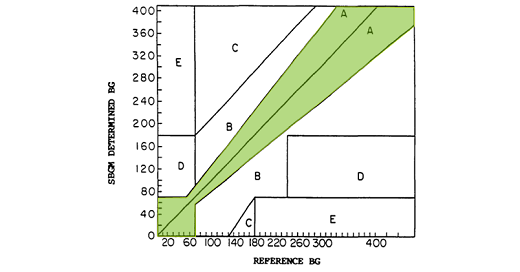
\includegraphics[width=0.75\textwidth]{images/cega.png} 
        \caption{
         A visualisation of the CEG \cite{cegaimage}
        }
      \end{figure}

      The approaches we have seen so far have all suffered from one common issue - a lack of data to train models on. In typical machine learning problems, datasets often consist of millions of datapoints which allows the creation of very complex and accurate models. In contrast, CGM datasets are difficult to create, and often consist of only thousands of datapoints which leads to a distinct shallowness in the data and inhibits the training of more accurate models. Aliberti et al. \cite{paper9} sought to rectify this issue and instead of just training their model on the data of one patient, they trained their model on the data of many patients - whilst keeping a large chunk of the training data as the data of the main patient in question. They claimed that this would not only make more data available for the training of the model but also make their model more flexible. Past approaches that are only trained on a single patient's data require a lot of fine tuning and produce a model that is rigid and can only be used on one specific T1DM patient. In medical practice, it would be infeasible to produce an individual model for every T1DM patient and, as such, Aliberti et al. \cite{paper9} claimed that their model, which would be trained across many different datasets, could offer a solution to this issue. They tried their attempt using both a Non-Linear Autoregressive NN (NAR), a network which computes the value of a signal $y$ at time $t$ using $n$ past values of $y$ as regressors, thus allowing it to model the dependency between sequential datapoints, and a LSTM RNN. Over 30, 45, 60 and 90 minute PHs, the NAR achieved RMSE of 18.2, 25.31, 33.12, 47.64 mg/dL respectively, and the LSTM received an RMSE of 5.93, 7.18, 13.21 and 28.57 mg/dL respectively. The LSTM was far more accurate than the NAR, and over a short PH this approach performed very well, but once again the performance very quickly dropped off at longer PH. 

      \subsection{Alternative Approaches}

      So far all of the approaches have viewed the task of BG Prediction as a regression task where you are trying to predict a value for the BG variation over the PH. Zhu et al. \cite{paper7} instead formulated the problem as a classification problem, where the change between current glucose value and the future glucose value is quantised into 256 different classes to be predicted between. The data was sourced from the OhioT1DM dataset \cite{ohio}, which is a dataset of real-life diabetes patients. Zhu et al. used a Convolution Neural Network (CNN) \cite{whatiscnn} a type of neural network typically used in image recognition, due to its ability to reduce the dimensionality of input data. Over a 30 minute PH, the approach achieved an average RMSE of 21.72 mg/dL for its predictions, which is not as promising as other approaches we have seen involving regression via an RNN. Another approach not using the traditional RNN was experimented with by Wang et al. \cite{paper10}, who built a model based on LightGBM \cite{lightgbm} - a gradient boosting algorithm that generates a decision tree to make predictions on the data. Over a 30 minute PH, they achieved a RMSE of 0.7721 mmol/L, which just falls within the range of accurate predictions, showing that the approach has merit at shorter prediction horizons.

	\subsection{Conclusions}
      In summary, we have seen a variety of different approaches to performing BG prediction using neural networks with various levels of success. Some approaches incorporated a large number of factors as well as CGM data, whilst others included more factors relating to the CGM data itself such as maximum and minimum points. However, despite all of these differences, all of the approaches shared in common that the performance dropped of quickly as the PH grew longer as well as the fact that they had not been trialed at all in an in vitro scenario. Coupling this lack of in vitro testing, along with the fact that approaches used a myriad of different datasets makes it very hard to say whether one approach is better than another, despite the common RMSE metric, or whether the dataset they were using lent itself towards being much easier to be predicted over; either due to a more gradual nature in the change of BG levels, or a better quality of data. 

      To rectify the second of these issues, some of these researched approaches and their features will be selected and implemneted using a consistent dataset - the OhioT1DM dataset \cite{ohio}. Through the use of a common dataset, there will be a common platform by which we can judge the performance of these different methods over differing prediction horizons.

%%%%%%%%%%%%%%%%%% SECTION 3 %%%%%%%%%%%%%%%%%%
\section{Methodology} % edit section heading as appropriate
    \subsection{Introduction}
      
    The flow chart below details the main aspects of the project and the pipeline in which they fit together. The data is first read from the OhioT1DM dataset using pandas before multiple levels of preprocessing occur to generate new signals from the input data. This new data is then split into windows based on the PH being predicted over, and models are built then optimised on the data. Finally, the models are evaluated using a number of metrics and visualisations are produced from these different metrics.

    \begin{figure}[H]
      \centering
      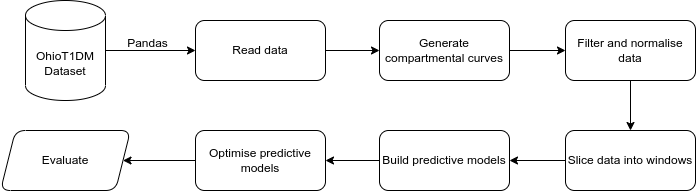
\includegraphics[width=\textwidth]{images/codeflow.png} 
      \caption{
       A flow chart detailing the main parts of the project
      }
    \end{figure}

    To implement the project, a python3 jupyter notebook development environment was used. A variety of different libraries were used, the most prevalent of which being listed below:
    \begin{itemize}
      \item pandasobsidian://open?vault=COMPSCI%20YEAR%203&file=Third%20Year%20Project%20-%2030040%2FOhioT1DM%2FDataFormatPaper.pdf
      \item numpy
      \item tensorflow
      \item matplotlib
      \item sklearn
      \item pickle
      \item keras tuner
    \end{itemize}
  
	\subsection{Detail}
        Tell story of the development of the models, from data processing to choices made in model hyperparameters / cleaning etc.

      \subsection{OhioT1DM Dataset}
      The OhioT1DM \cite{ohio} dataset is a dataset developed to assist in the research of blood glucose level prediction. It consists of 8 weeks of CGM data taken every 5 minutes for 12 different patients with T1DM. Alongside the CGM data are a number of events of interest such as when a patient had a meal and the amount of carbohydrate consumed, or when a patient injected themselves with a dose of insulin. There are 20 such factors included in the dataset. The data for the patients is split into training examples and testing examples and for each patient there are ~13,000 samples split across the two sets. The patient data is held in XML files and approval to use the dataset was obtained through The University of Manchester.

      The data in the dataset was gathered from two separate cohorts - one cohort in 2020 and the other in 2018. For the purpose of this project, we will be using the data from 3 randomly selected patients from the 2018 cohort. Information about the selected patients can be seen in the table below.


      \begin{table}[H]
        \begin{center}
          \caption{A table showing individual information about the selected patients}
          \begin{tabular}{||c c c c c||} 
          \hline
          ID & Gender & Age & Pump Model & Sensor Band \\ [0.5ex] 
          \hline\hline
          563 & Male & 40-60 & 530G & Basis \\ 
          \hline
          570 & Male & 40-60 & 530G & Basis \\
          \hline
          588 & Female & 40-60 & 530G & Basis \\ [1ex]
          \hline 
          \end{tabular}
        \end{center}
      \end{table}

      As we can see from this table, there are two male patients and one female patient; with all of the patients being between 40-60 years of age. The model of the insulin pump that the patients used as well as the type of sensor band (a sensor used to record data such as heart rate) are also included for each patient. These data, whilst useful to fine-tuning predictions made on their respective fields were ignored for this experiment as no data relating to the sensor band was utilised, and fitting insulin curves to the specific pump model was deemed to reduce the flexibility of the model by specifying it to one kind of pump.

      \subsection{Reading in the Data}

        \subsubsection{Data storage format}
          As mentioned earlier, all of the data for the patients is stored in XML files. Each individual field of data for the patient (e.g. the CGM data) is stored within an individual object that consists of a list of events of a time when the event occurred, and a value for the event.

          \begin{figure}[H]
            \centering
            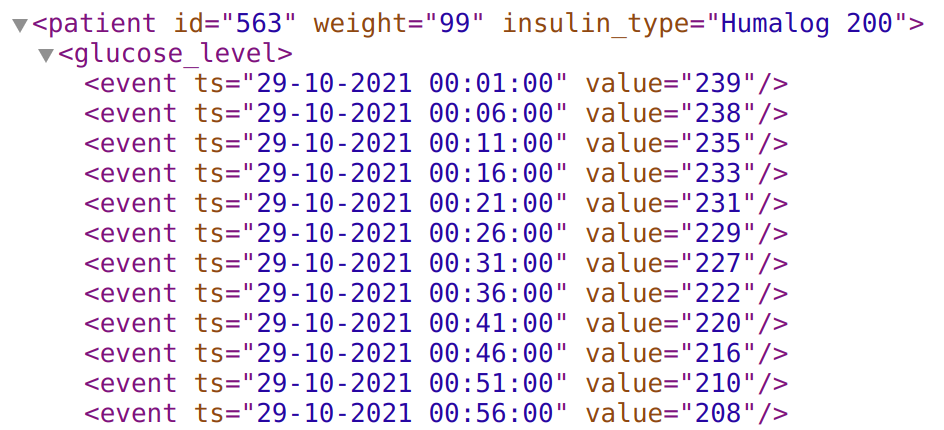
\includegraphics[width=0.5\textwidth]{images/XMlFile.png} 
            \caption{
             An image showing a short extract of data for patient 563
            }
          \end{figure}
          
        \subsubsection{}

      \subsection{Generating Compartmental Curves}

      \subsection{Filtering and Normalisation}

      \subsection{Range Slicing}

      \subsection{Building the Models}

      \subsection{Model Optimisation}
	
	\subsection{Summary}
        Provide a brief summary of development that leads on to results of the experiments performed.


%%%%%%%%%%%%%%%%%% SECTION 4 %%%%%%%%%%%%%%%%%%
\section{Results and discussion} % edit section heading as appropriate
    \subsection{Introduction}
        Briefly introduce results section, talk about metrics we are going to use etc.
	
	\subsection{Detail}
        Show different metrics and graphs e.g. table of RMSE across different time spans for different models, plots of metrics vs hyperparameter settings / regularised vs not regularised etc.
	
	\subsection{Summary}
        Provide a brief summary of the results seen and what they show us

% Add more sections if necessary


%%%%%%%%%%%%%%%%%% SECTION 5 %%%%%%%%%%%%%%%%%%
\section{Conclusions and future work} % edit section heading as appropriate
    \subsection{Conclusions}
        Talk generally about the parallels and differences seen from my approach vs the approaches studied in the literature review. Explain limitations of the task in reality.
	
	\subsection{Future work}
        Go into detail about how the model could be improved / what it would take to put such a model out into the real world via CGM/Pump.
    


%%%%%%%%%%%%%%%%%% REFERENCES %%%%%%%%%%%%%%%%%%
%\clearpage % uncomment to start on a new page if wanted
\printbibliography[title={References},heading=bibintoc] % a single list of references for the whole thesis



%%%%%%%%%%%%%%%%%% APPENDICES %%%%%%%%%%%%%%%%%%
\begin{uomappendix} 
    \section{Project outline}
    Project outline as submitted at the start of the project is a required appendix. Put here. 
    
    \section{Risk assessment}
    Risk assessment is a required appendix. Put here.

    %\section{Other appendices as necessary}
\end{uomappendix}


%%%%%%%%%%%%%%%%%% END MATTER %%%%%%%%%%%%%%%%%%
\end{document}